\documentclass{scrreprt}
\usepackage[french]{babel}
\usepackage[utf8]{inputenc}
\usepackage{listings}
\usepackage{underscore}
\usepackage[bookmarks=true]{hyperref}
\hypersetup{
    bookmarks=false, % show bookmarks bar?
    pdftitle={Projet SASIAE}, % title
    pdfauthor={Raynal Jean-Raymond, Dauphin Loïc, Clément Lansmarie, Hugo Brunie, Nicolas Belin, Benoit Gilbert, Théotime Méralli-Ballou}, % author
    pdfsubject={TeX and LaTeX}, % subject of the document
    pdfkeywords={TeX, LaTeX, graphics, images}, % list of keywords
    colorlinks=true, % false: boxed links; true: colored links
    linkcolor=blue, % color of internal links
    citecolor=black, % color of links to bibliography
    filecolor=black, % color of file links
    urlcolor=purple, % color of external links
    linktoc=page % only page is linked
}%1 
\def\myversion{}
\title{%
\flushright
\rule{16cm}{5pt}
\vskip1cm
{\Huge Projet SASIAE}\\
\vspace{10cm}
{\small Théotime Méralli-Ballou\\ Raynal Jean-Raymond\\ Clément Lansmarie\\ Benoit Gilbert\\ Dauphin Loïc\\ Nicolas Belin\\ Hugo Brunie\\ }
\vfill
\rule{16cm}{5pt}
}
\date{}
\usepackage{hyperref}

\begin{document}

\maketitle
\tableofcontents

\chapter{Introduction}

%% TODO : Préciser qu'EIBROT utilise des AVR

\section{Objectifs}

    Eirbot est une association qui conçoit des robots pour participer à la coupe de France de robotique. Celle-ci consiste à opposer de deux à quatre robots autonomes qui interagissent avec les différents objets sur une table dans le but de marquer un maximum de points. L'association a besoin de fiabiliser les robots, via plus de tests et une meilleure compréhension du comportement du robot. Un simulateur permettra de mieux comprendre l'enchainement du code et ainsi cibler les erreurs d'exécution plus rapidement qu'une mise en scéne réelle.
    Le simulateur développé ici doit pouvoir reproduire une situation de jeu et interagir avec le code pour repérer le comportement des robots.
    
    
\section{Etendue du Projet et Spécification du produit}


%% dire que le projet est séparé en API, GUI et simulateur mais quelle ne prend pas en compte le code robot. déscription du livrable : combien d'exécutable ? la manière de l'utiliser ? et sinon je sais pas trop ce qu'il faut dire ici. des idées ?



%%%%%%%%%%%%%%%%%%%%%%%%%%%%%%%%%%%%%%%%%%%%%%
      \chapter{Description générale}        %%
%%%%%%%%%%%%%%%%%%%%%%%%%%%%%%%%%%%%%%%%%%%%%%
\newpage
\section{Besoins de l'API}
\subsection{Besoins foncionnels}

Le but de l'API est de faciliter la programmation d'un robot.

\subsubsection{Gestion des entrées sorties du robot}

Le robot est composé de différents capteurs et actionneurs, le but de l'API est de proposer des interfaces pour intérargir avec ces éléments, en permettant de ne pas avoir à se soucier de l'architecture matérielle.

\subsubsection{Gestion des modules du microprocesseur}

Tous les microprocesseurs proposent plus ou moins les mêmes services. Il faut pouvoir les configurer sans avoir à connaitres les registres à modifier.

\subsubsection{Détecter les erreurs d'opération}

Le manque de mémoire et de puissance de calcul sur les AVR utilisés à Eirbot nous poussent à contrôler et réduire la taille des entiers utilisés. Cela augmente donc les chances de produire des overflows lors des opérations, qui sont difficilement détectables sur une architecture PC de 32 ou 64 bits. En effet, les registres du processeur étant plus grand, si la suite d'opération ammenant l'overflow aboutit à un résultat compris dans les limites du type de départ, l'overflow n'aura pas lieu sur un PC.

Ces overflows ont de graves conséquences dans le comportement du robot. De ce fait, il est important d'avoir un mécanisme de détection de ces erreurs d'opérations arithmétiques lors de la simultation.

La solution retenue est de passer par des classes qui ré-implémentent les types utilisés afin d'en surcharger les opérations. De cette manière toutes les étapes du calcul sont maitrisées par l'API.

Dans le cas d'une erreur, un message sera envoyé au simulateur pour en avertir l'utilisateur.

\subsubsection{Planification des tâches}

Sur les robots, nous avons besoin de pouvoir exécuter des routines à intervalle régulier (une routine pour détecter la présence d'un obstacle afin d'arrêter les moteurs par exemple). C'est pourquoi nous avons besoin d'un planificateur de tâches. Celui ci devra nous permettre :
\begin{itemize}
    \item d'ajouter une nouvelle routine avec l'intervalle de temps entre chaque appel ainsi que sa priorité ;
    \item de supprimer une routine du planificateur ;
\end{itemize}

\subsection{Besoins non fonctionnels}

\subsubsection{Langage de programmation}

Le langage de programmation choisi est le C++. C'est celui qui répond le mieux à nos attentes. En effet l'API est pensée à l'aide des mécanismes objet. Le C++ est un langage orienté objet qui s'adapte donc plus que le C au développement de l'API, notemment pour la surcharge des opérateurs pour détecter les overflows. De plus nous avons besoin d'un code qui puisse s'adapter aux différentes architectures de micro-contrôleur, afin de posséder cette généricité nous pouvons avec le langage C++ utiliser le mécanisme des \og templates \fg qui est adapté. Enfin nous écartons le JAVA, car même s'il est orienté objet il est souhaitable de garder la compatibilité avec le code Robot qui en en langage C.

\subsubsection{Compatibilité AVR - x86}

La même API est utilisée pour la simulation sur PC et pour le robot. Il est proposé de la séparer en 3 parties principales :
\begin{itemize}
    \item{La partie indépendante de l'architecture.}
    \item{La partie dépendante de l'architecture, côté simulation.}
    \item{La partie dépendante de l'architecture, côté AVR.}
\end{itemize}

\subsubsection{Taille des executables}

L'architecture actuellement utilisée n'offre dans le meilleur des cas que 128 Ko de mémoire flash destinée à stocker l'exécutable, et 4 Ko de RAM. Il faut donc être capable de générer un code le plus léger possible.




\newpage
\section{Besoins du Simulateur}

\subsection{Besoins fonctionnels}

Le but premier du simulateur est de vérifier le comportement de un ou plusieurs robots sur une table type coupe de France de robotique avec un retour sur l'exécution afin d'adapter, plus tard, le code robot aux erreurs de capteurs. Notre simulateur SASIAE n'a donc pas pour but de tester l'efficacité
% ligne suivante rajoutée par Clément %
(en terme de rapidité de calcul)
du code robot mais bien 
% ligne suivante rajoutée par Clément %
son intelligence et
comment celui-ci réagit aux données erronnées envoyées par les capteurs, ou aux évènements imprévus pouvant se produir.

On veut pouvoir :
\subsubsection{Exécuter une simulation}
Le simulateur doit bien entendu pouvoir lancer une simulation et la mettre en pause en effet l'utilisateur peut vouloir analyser pas à pas une simulation. De plus l'utilisateur doit pouvoir Sauvegarder et Charger une simulation afin de pouvoir la rejouer à un autre moment.

\subsubsection{Enregistrer la simulation}
%N ET T
Pendant l'exécution de la simulation, il sera possible de déclencher l'enregistrement de la simulation. Les enregistrements permettront de rejouer une simulation sans posséder le code robot de base, ni sa position initiale. Ainsi, tous les logs d'exécutions seront enregistrés, afin de compléter ces informations, la position du robot sera enregistrée petit à petit selon une fréquence optimale.

\subsubsection{Lire une simulation}
%N ET T
A l'aide d'un enregistrement d'une simulation, le simulateur peut rejouer la simulation sans le code robot. Les logs permettent de définir la vitesse et sa position fera office de garde fou pour éviter une imprécision/vérifier l'exécution.

\subsubsection{Simuler le scénario}
%N ET T
Le simulateur doit pouvoir exécuter un scénario de manière déterministe, en laissant la posibilité à l'utilisateur de faire intervenir des erreurs artificielles sur les données renvoyées par les capteurs.

\subsubsection{Simuler un environnement 3D}
Le déplacement des robots sur table est entièrement dépendant de la physique et de l'état de son environnement en temps réel. Il faut donc que le simulateur puisse gérer cet environnement et les contraintes physiques qu'il engendre. Cela implique la détection des adversaires, la détection des objets ou les situations aléatoires de blockages dues à la position d'un objet mobile non prévue. %%fin de phrase vraiment à revoir...%%

\subsubsection{Représenter un environnement en 2D}
L'affichage se fera en deux dimensions. Nous souhaitons pouvoir représenter les robots en vue de dessus, donc le simulateur devra afficher une projection du retour du moteur physique procédant à la simulation proprement dite. 

\subsubsection{Charger une table}
La table de jeu est l'élément le plus important de l'environnement. Elle contient toutes les contraintes immobiles mais aussi la position des éléments mobiles (éléments de jeu). De plus, son prototype change chaque année. Il faut donc pouvoir la changer facilement. Pour cela un langage de description a été créé, présenté dans la partie dédiée de ce document.

\subsubsection{Le choix des robots}
%HUGO
Les robots sont bien sûr le coeur de la simulation. On doit pouvoir en charger entre 1 et 4 afin de simuler l'environnement (en plus de la table). Les robots peuvent évoluer assez rapidement. Ainsi, d'une semaine sur l'autre l'architecture d'un robot peut être complétement refaite. C'est donc l'élément qui sera changé le plus souvent. Donc l'utilisateur pourra charger son robot à partir d'un navigateur de son systême de fichier (le code de description de la structure du robot est au format XML, voir \ref{desc_robot}). Le simulateur devra comprendre quelques exemples de fichiers de description de robot. Finalement, une fois le fichier de description chargé, l'utilisateur devra choisir l'exécutable du code robot associé, l'équipe à laquelle celui-ci appartiendra (équipe 1 ou équipe 2) et sa position initiale. 

\subsubsection{Gérer les objets}
De même que les robots, on veut insérer des éléments externes à l'environnement (et non-prévus par celui-ci). Tels que des balles de ping pong perdues par un robot au cours d'un action balistique. On doit donc pouvoir insérer, déplacer et supprimer des objets dans l'environnement de jeu.

\subsubsection{Tracer l'exécution, journaliser les événements et afficher l'état des capteurs}
Le simulateur est un outil de développement de programme pour robot. Ainsi, on veut pouvoir avoir accès à la trace d'exécution du code ou au moins à une journalisation de l'exécution. De plus, on veut pouvoir obtenir les informations détectées par le robot et non-visibles sur l'affichage 2D telles que le patinage, les erreurs d'overflow ... cette liste est non-exhaustive et pourra être complétée plus tard. De même, les valeurs envoyées par les capteurs doivent apparaitrent en temps réel.

\subsubsection{Simuler des capteurs}
%N ET T
Les objets qui représentent les entrées et sorties du robot dans l'API ont besoin de leurs homolgues dans le simulateur afin que le robot puisse avoir connaissance de son environnement. Il faut donc calculer pour ces objets les différentes valeurs qui doivent être envoyées, à partir du simulateur physique. Il n'est pas envisageable d'implémenter tous les capteurs existants, il faut donc proposer une solution générique paramétrable par l'utilisateur final qui doit avoir la possibilité d'utiliser un nouveau capteur, qui sera ajouté à une bibliothèque dynamique contenant les capteurs existants, l'utilisateur doit préciser dans la description du robot les atributs de la classe choisie dans la bibliothèque. Les calculs de valeur sont réalisés par la bibliothèque. En cas de simulation d'erreur, soit celle-ci est due à la possibilité d'erreure du capteur, elle est prise en compte dans la bibliothèque, soit elle est voulue ponctuellement par le coordinateur. Les capteurs doivent donc être organisés le plus précisemment possible en fonction des données retournées, par exemple si elles sont numériques, analogiques, binaires; et si le capteur mesure une distance, un champs électromagnétique, une pression...
Le coordinateur est le module central, il relie les capteurs définis par les bibliothèques dynamiques et le moteur physique au socket, dans lequel il inscrit la valeur calculée.
%il faudra préciser EXACTEMENT quels sont les classes de capteurs et par exemple classer les capteurs que le robot d'eirbot utilise actuellement pour montrer que le classement est pertinent.


\subsubsection{Simuler des actionneurs}
%N ET T
Le coordinateur reçoit les commandes envoyées par l'API Aversive++ et les transmet aux actionneurs, comme le servo-moteur ou le moteur courant-continu. Ensuite ces actionneurs interprètent la commande. S'ils reçoivent une commande correcte, ou si au contraire la commande n'entre pas dans les spécifications du servo-moteur un message est envoyé au coordinateur, celui-ci communique l'information au GUI qui renseigne si le signal est erroné, ou l'angle auquel se situe le palonnier du servomoteur dans le cas d'une bonne commande.

Quant aux moteurs de propulsion du robot, la simulation a besoin d'être plus complète. En effet, il est très important pour EIRBOT que le robot ait une trajectoire la plus précise possible.
%CECI NE VEUT RIEN DIRE -> (JR)% moteur recoit commande de coordinateur . il envoit résultat au moteur physique qui renseigne l'affichage (GUI) et les roues codeuses %(A TRAVERS LE COORDINATEUR ??? ) 
%******************************************************************************%
% Pagagraphe à réécrire JR
On va donc simuler les roues codeuses qui mesurent le déplacement effectif du robot sur la table par rapport à une position initiale déterminée.
Prenons l'exemple d'un robot qui rencontre un obstable et patine car il est bloqué par celui-ci. L'API Aversive ++ envoit le signal "avance" au coordinateur, qui le transmet à l'émulateur du moteur. Ce dernier envoie un message au moteur physique pour signaler le mouvement du robot. Le robot ne bouge plus, mais ses roues patines. Le moteur physique renseigne en continu les roues codeuses qui touchent le sol, celle-ci renvoit un signal "j'avance de 0" au coordinateur qui le fait suivre à l'API. Et c'est au code du robot de traiter ce problème.
%******************************************************************************%

\subsubsection{Communiquer avec l'API}
%N ET T
Comme il a été évoqué dans les paragraphes précédents, le coordinateur doit pouvoir communiquer avec l'API et l'interface graphique. La communication avec l'API se fait par le biais d'un socket, avec un socket par exécutable de code robot. À chaque pas de simulation, le moteur physique envoie un signal de fin du pas, puis l'interface graphique récupère le nouvel état de simulation pour rafraichir l'affichage ainsi que les messages à l'utilisateur.
   
\subsection{Besoins non fonctionnels}

\subsubsection{Simuler la physique de l'environnement}
Simuler à l'aide d'un moteur physique les interactions entre objets notament les collisions en 3 dimensions. La récupération d'un objet par le robot ne sera pas simulé. Le moteur physique devra par ailleur gérer les collisions le plus simplement possibles (sans avoir à diminuer le pas simulation à l'approche d'un objet).

\paragraph{Le choix du moteur physique}
Nous avons testé le moteur Bullet sur un exemple : une sphère solide qui tombe sur un sol solide, celle-ci s'enfonce d'au pire le sixième de son diamètre.
% je continue à penser que ce paragraphe n'a rien à faire dans le document



\newpage
\section{Architecture}
%%%% Clément %%%%
\label{architecture}

Le développement de l'application sera découpé en plusieurs parties :
\begin{itemize}
    \item le GUI se chargera de l'interaction avec l'utilisateur ;
    \item le moteur physique s'occupera de simuler l'environnement physique ;
    \item le coordinateur s'occupera :
    \begin{itemize}
        \item de charger les bibliothèques dynamiques simulant les différents modules physiques et mécaniques ;
        \item d'interpréter le fichier de description de la table pour la charger dans le moteur physique ;
        \item d'interpréter le fichier de description d'un robot pour le modéliser dans le moteur physique, de lancer son ou ses exécutables, d'établir la communication avec les processus ainsi créés et d'instancier les différents modules nécessaires pour ce robot ;
        \item de journaliser certains évenements de la simulation ;
    \end{itemize}
\end{itemize}

Aversive++, implémentation\_simulation sera, quant à elle, linkée lors de la compilation avec le code robot et elle s'occupera de la communication avec le coordinateur.

Elle comportera un \texttt{Client} "de coordination" qui s'occupera de récupérer les messages du coordinateur de manière asynchrone par rapport au code robot, mettre à jour les données de capteurs, ainsi que gérer l'execution des tâches enregistrées dans les schedulers (voir partie\ref{planif_taches} Planification des tâches) .

Au sein de l'application :
\begin{itemize}
    \item le GUI communiquera avec le coordinateur et le moteur physique pour récupérer et afficher une vue de l'environnement physique, la ou les valeurs des capteurs et afficher le journal de la simulation ;
    \item le coordinateur et le moteur physique intéragiront ensemble afin que les différents modules puissent calculer leurs valeurs (dans le cas de capteurs) ou modifier des valeurs (dans le cas d'actionneur) ;
\end{itemize}

%%%%%%%%%%%%%%%%%%%%%%%%%%%%%%%%%%%%%%%%%%%%%%%%%%%%%%%%%%%%%%%%%%%%%%%%%%%%%%%
%%% Je touve les deux figure redondantes et la secondes est plus complète et plus agréable à regarder. JR
%%% +1 (Loïc)

%\vspace{5 mm}
%\begin{figure}
%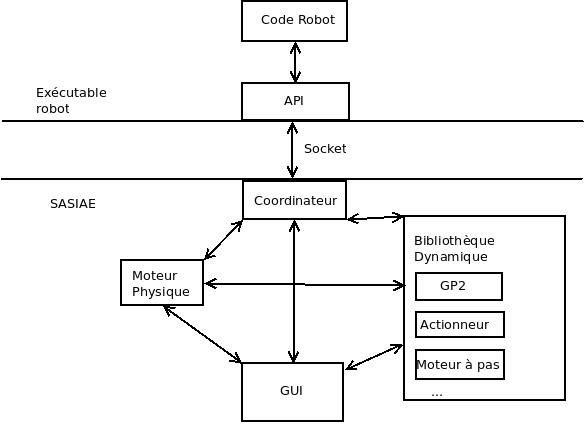
\includegraphics[scale=0.80]{architecture.png}
%\caption{shéma de l'architecture globale de SASIAE}
%\label{figurearchitecture}
%\end{figure}
%\vspace{5 mm}

%\newpage

La figure \ref{messagearchitecture} présente de façon un peu plus détaillée les messages envoyés entre les différents composants du simulateur.
L'objet "Module" est un module générique qui peut être un capteur et un actionneur, il y aura dans l'application plusieurs modules, mais le schéma 
n'en comporte qu'un pour des soucis de lisibilité.

%% Clément : C'est quoi ce "ClientCoordination" côté exécutable robot qui reçoit les valeurs des capteurs ? C'est Aversive++ qui est aussi censé gérer et fournir une abstraction des capteurs !!!

\begin{figure}
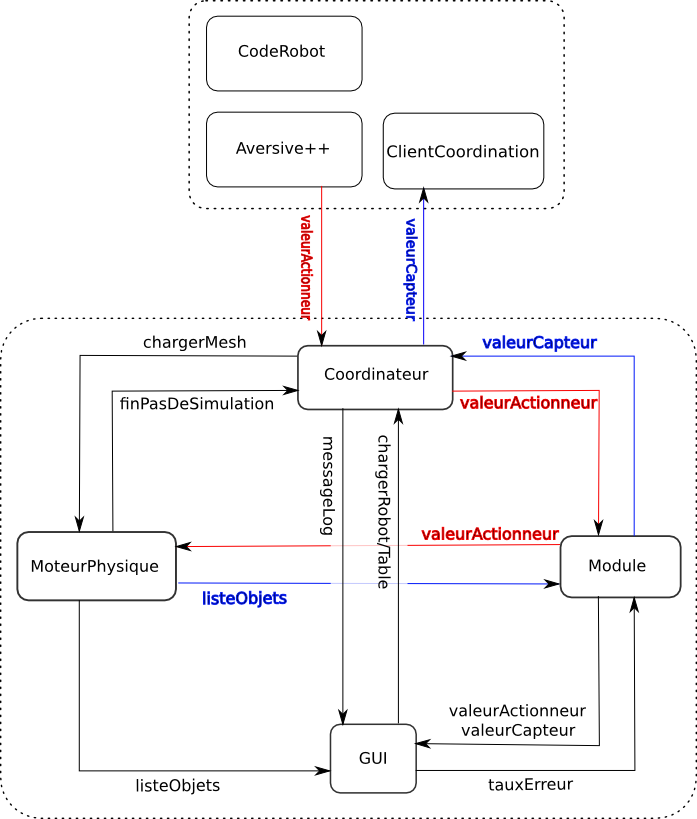
\includegraphics[scale=0.70]{architecturemsg.png}
\caption{messages entre les composants de l'architecture}
\label{messagearchitecture}
\end{figure}
\vspace{5 mm}


\newpage
\chapter{Conclusion}

\newpage
\section{Évolution envisagées}

\newpage
\section{Validation de l'application}

\newpage
\section{Planning}



\end{document}